\documentclass{article}
\usepackage[utf8]{inputenc}
\usepackage{amsmath,amsfonts,graphicx,mathtools,framed,siunitx,parskip}
\usepackage[noabbrev]{cleveref}

\usepackage{cancel}

% Set up the header
\usepackage{fancyhdr}
\rhead{}
\pagestyle{fancy}
\lhead{Physics 374B Notes}
\rhead{Fall 2020}
\cfoot{\thepage}

\usepackage{framed}
\usepackage{xcolor}
\let\oldquote=\quote
\let\endoldquote=\endquote
\colorlet{shadecolor}{orange!12}
\renewenvironment{quote}{\begin{shaded*}\begin{oldquote}}{\end{oldquote}\end{shaded*}}

\begin{document}

\section*{The Wave Equation}

We are familiar with the motion of a coupled oscillator; that is, two blocks suspended by three springs. 

\begin{figure}[h]
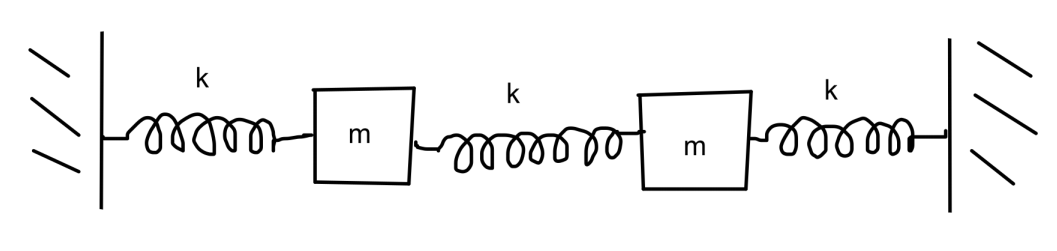
\includegraphics[width=10cm]{coupled-oscillators.png}
\centering
\end{figure}

Instead of two springs, let's now consider $N$ blocks suspended by $N+1$ springs. (Of course, in the limit of large $N$, we will take $N\approx N+1$.) Each block has mass $m$. Each spring has spring constant $k$ and natural length $\ell$. 

Let $u_i$ indicate the displacement of the $i^\text{th}$ block from equilibrium. Then we can calculate the forces on that block based on its position and the positions of its neighbors:
$$
m \ddot{u_i} = -k \; \left( u_i - u_{i-1} \right) - k \; \left( u_i - u_{i+1} \right)
$$
Let's quickly confirm that our signs are correct. If the ${i-1}^\text{st}$ block is displaced in the positive direction, $u_{i-1}$ is positive, and the force on $u_i$ should be positive. If the $i+1^\text{st}$ block is displaced in the positive direction, $u_{i+1}$ is positive, and the force on $u_i$ should be positive. 

We are interested in the limit of very large $N$, at which point the terms above look a lot like derivatives. Specifically:
\begin{align*}
    u'_{i-1/2} &= \lim_{N\rightarrow\infty}\frac{u_i - u_{i-1}}{\ell}&
    u'_{i+1/2} &= \lim_{N\rightarrow\infty} \frac{u_{i+1} - u_i}{\ell}
\end{align*}
Furthermore, those two first derivatives look an awful lot like a second derivative:
$$
u''_i = \lim_{N\rightarrow\infty} \frac{u_{i+1/2} - u_{i-1/2}}{\ell}
$$
As long as we're taking derivatives, we may as well swap out the discrete $u_i(t)$ for a continuous function $u(x, t)$. The whole expression then looks like:
$$
m \, \ddot{u} = k \ell^2 \, u''
$$
The quantities $k$, $\ell$, and $m$ all become problematic in the limit of large $N$, but each can be related to a macroscopic quantity:
\begin{align*}
    k &= KN &
    \ell &= L/N &
    m &= M/N
\end{align*}
Where $L$ is the length of the entire slinky (or jumprope, or whatever we're modeling), $K$ is its spring constant, and $M$ is its mass\footnote{The scaling of mass and length are clear, but the spring constant may be less so. Suppose we glue together ten springs with $k=\SI{1}{\newton/\m}$. If we put \SI{1}{\newton} of tension on that spring, it'll stretch ten meters.}. Plugging those into the equation of motion, the $N$ all cancel, and we're left with:
\begin{align*}
    \ddot{u} &= \frac{KL^2}{M} u''
\end{align*}
We may also note that $\tfrac{KL^2}{M}$ has units of velocity squared. For brevity, let's call it $c^2$. This gives us the one-dimensional wave equation:
\begin{align*}
    \ddot{u} &= c^2 u''&
    &\text{or equally}&
    \frac{\partial^2}{\partial t^2} u(x, t) &= c^2 \frac{\partial^2}{\partial x^2} u(x, t)
\end{align*}

\section*{A Sum of Waves}

Our system is made out of blocks and springs, so we may reasonably guess that its motion will be described by sines and cosines. This can be proved using separation of variables, which is beyond the scope of the present exercise. For the moment's we can easily enough verify that the following satisfies the wave equation as long as $ck = \omega$:
\begin{align*}
    u(x, t) &= 
        \alpha \sin (kx) \cos (\omega t) +
        \beta \sin (kx) \sin (\omega t) + 
        \gamma \cos (kx) \cos (\omega t) +
        \delta \cos (kx) \sin (\omega t)
\end{align*}
Four terms is a bit much, so let's get rid of a few of them using boundary conditions. Our slinky is anchored at both ends, so ${u(0, t)=u(L, t)=0}$. So we don't want any $\cos(kx)$ terms. Let's also say that the slinky is initially at rest; we have deformed it, then we let it go at $t=0$. So $\dot{u}(x, 0)=0$, meaning we don't want any $\sin(\omega t)$ terms either. We're left with:
\begin{align*}
    u(x, t) &= 
        \alpha \sin (kx) \cos (\omega t)
\end{align*}
Where $\alpha$ is the wave amplitude, $\omega$ is its frequency, and $k$ is its wavenumber ($k=\tfrac{2\pi}{\lambda}$, where $\lambda$ is the wavelength). 

This expression describes a single standing wave. For a general solution, then, let's look at a linear combination of standing waves. This is more or less the same thing we did with the coupled oscillators, though in that case there were only two waves to worry about. In this case, there are many:
\begin{align*}
    u(x, t) &= \displaystyle\sum_n \alpha_n \sin \left( k_n x \right) \sin \left( \omega_n t \right)
\end{align*}
As a sanity check, let's plug back into the wave equation:
\begin{align*}
    \ddot{u} &= c^2 u'' \\
    \displaystyle\sum_n -\alpha_n \omega_n^2 \sin \left( k_n x \right) \cos \left( \omega_n t \right)
    &= 
    c^2 \displaystyle\sum_n -\alpha_n k_n^2 \sin \left( k_n x \right) \cos \left( \omega_n t \right) \\
    \displaystyle\sum_n \alpha_n \left[ \omega_n^2 - c^2 k_n^2 \right] \sin \left( k_n x \right) \cos \left( \omega_n t \right)
    &= 0  
\end{align*}
The amplitudes $\alpha_n$ may vary arbitrarily and independently, so this expression can be true only so long as the bracketed expression is zero, or $\omega_n=ck_n$.

From here, we can figure out what $\omega_n$ and $k_n$ look like. Recall that the edges of our slinky are fixed, ${u(0)=u(L)=0}$, so $k_n L$ must always be an integer multiple of $\pi$. That leaves us with:
\begin{align*}
    k_n &= \frac{n \pi}{L} &
    &\text{and so}&
    \omega_n &= ck_n = \frac{n \pi c}{L}
\end{align*}

\section*{Fourier Series}

We now have a general expression for a longitudinal wave on a slinky with fixed ends, which is momentarily at rest at $t=0$: 
\begin{align*}
    u(x, t) &=
    \displaystyle\sum_n \alpha_n \sin \tfrac{n \pi x}{L} \cos \tfrac{n \pi ct}{L}
\end{align*}
Our final step is to figure out the amplitudes $\alpha_n$ to line up with our initial conditions. To do so, we need a pair of asides. 

\begin{quote}
\textbf{Fourier's Theorem}

Let $U(x)$ be a function defined on the domain $x=0$ to $x=L$, with ${U(0)=U(L)=0}$. Then there exist some set of amplitudes $\left\{ \alpha_n \right\}$ such that:
\begin{align*}
    U(x) &= \displaystyle\sum_n \alpha_n \sin \left( \tfrac{n\pi x}{L} \right)
\end{align*}
In other words, as long as the boundary conditions line up, any function $U(x)$ can be constructed from a linear combination of sine waves.

Proof of Fourier's theorem is beyond the scope of the present exercise. Hopefully you at least find it plausible.
\end{quote}

\begin{quote}
    \textbf{Sine Waves are Orthogonal}

    Much like eigenvectors are always perpendicular to one another, sine wave ``eigenfunctions'' are also orthogonal, in that their inner product is zero unless they're the same. Since we are dealing with continuous functions, the inner product is an integral rather than a dot product:
    $$
    \frac{2}{L}
    \displaystyle \int_0^L \sin \left( \tfrac{m \pi x}{L} \right) \sin \left( \tfrac{n \pi x}{L} \right) \, dx
    =
    \left\{
        \begin{array}{cl}
          1 & \text{if $m=n$} \\
          0 & \text{otherwise} \\
        \end{array}
        \right.    
    $$
    This can be proved using the angle addition formula:
    $$
        \cos \left( a \pm b \right) = \cos a \cos b \mp \sin a \sin b
    $$
    Then:
    $$
        \cos \tfrac{(m\pm n) \pi x}{L} = 
            \cos \tfrac{m \pi x}{L} \cos \tfrac{n \pi x}{L} \mp
            \sin \tfrac{m \pi x}{L} \sin \tfrac{n \pi x}{L} 
    $$
    Subtracting a pair of such expressions allows us to cancel the cosine terms, leaving only the sines:
    $$
    \tfrac{1}{2} \left(
    \cos \tfrac{(m-n) \pi x}{L} -
    \cos \tfrac{(m+n) \pi x}{L} 
    \right)
    = 
        \sin \left( \tfrac{m \pi x}{L} \right) \sin \left( \tfrac{n \pi x}{L} \right)
    $$    
    Rearranging our sines into cosines giives us an integral that can be evaluated directly:
    \begin{align*}
        \displaystyle \int_0^L \sin \tfrac{m \pi x}{L} \sin \tfrac{n \pi x}{L} \, dx &= \\
        \displaystyle \int_0^L \tfrac{1}{2} \left(
    \cos \tfrac{(m-n) \pi x}{L} -
    \cos \tfrac{(m+n) \pi x}{L} 
    \right) \, dx
    \end{align*}
    Where, for any integer $q \not= 0$:
    \begin{align*}
    \displaystyle \int_0^L \cos \tfrac{q \pi x}{L} \, dx &=
    \left[ \tfrac{L}{q\pi} \sin \tfrac{q \pi x}{L} \right]^L_0 \\
    &= \tfrac{L}{q\pi} \left( \sin q\pi - \sin 0 \right) \\
    &= 0
    \end{align*}    
    So the only nonzero term comes from the case $m=n$, since ${\cos \frac{0\pi x}{L}=1}$. 
\end{quote}
Let's suppose the initial displacement of the slinky is given by $U(x)$:
$$
u(x, 0) = U(x) = \displaystyle\sum_n \alpha_n \sin \tfrac{n\pi x}{L} \cancelto{1}{\cos \tfrac{n \pi c t}{L}}
$$
Notably, by looking at $t=0$, we don't have to worry about any of the time-dependent cosines. 

Then let's take the inner product of each side with $\sin \tfrac{m \pi x}{L}$. That is, let's multiply and integrate:
\begin{align*}
    U(x) &= \displaystyle\sum_n \alpha_n \sin \tfrac{n\pi x}{L} \\
    \displaystyle \int_0^L \sin \frac{m \pi x }{L} \, U(x) \, dx &=
    \displaystyle \int_0^L \sin \frac{m \pi x }{L} \, \displaystyle\sum_n \alpha_n \sin \tfrac{n\pi x}{L} \, dx \\
    &=
    \displaystyle\sum_n \alpha_n \displaystyle \int_0^L \sin \frac{m \pi x }{L} \,  \sin \tfrac{n\pi x}{L} \, dx \\
    &=
    \alpha_m \frac{L}{2} \\
\end{align*}
Note that all terms with $m \not= n$ are zero, so the sum collapses to a single term. We're left with a way to calculate $\alpha_m$ based on the initial perturbation of the slinky $U(x)$:
\begin{align*}
    \alpha_m &= \frac{2}{L} \displaystyle \int_0^L \sin \frac{m \pi x }{L} \, U(x) \, dx
\end{align*}
And let's take a moment to recall why we cared about the amplitudes $\alpha$ in the first place. This tells us not only the shape of the wave initially, but its evolution through time. Each amplitude $\alpha$ tells us the amplitude of one resonant mode. And for each mode, we already know the wavelength and frequency. So the complete motion of the wave is described by:
\begin{align*}
    u(x, t) &= \displaystyle\sum_n \alpha_n \sin \tfrac{n\pi x}{L} \, \cos \tfrac{n\pi c t}{L} &
    &\text{where}&
    \alpha_n &= \frac{2}{L} \displaystyle \int_0^L dx \, \sin \tfrac{n \pi x }{L}  \, u(x, 0) 
\end{align*}
Again, assuming fixed ends and no motion at $t=0$. To account for loose ends, we'd need cosine terms in $x$, and to allow initial velocity we'd need sine terms in $t$. 
\end{document}